% ~~~~~~~~~~~~~~~~~~~~~~~~~~~~~~~~~~~~~~~~~~~~~~~~~~~~~~~~~~~~~~~~~ %
\newif	\ifexternalize					%\externalizetrue			%
\newif	\ifshowonlynotes				%\showonlynotestrue			%
\newif	\ifhandout						%\handouttrue				%
\newif	\ifshowsolutions				%\showsolutionstrue			%
\newif	\ifshownotes					%\shownotestrue				%
%																	%
% enablers for conditional compiling through bash scripting			%
\ifdefined\EXTERNALIZE	\externalizetrue	\fi						%
\ifdefined\ONLYNOTES	\showonlynotestrue	\fi						%
\ifdefined\HANDOUT		\handouttrue		\fi						%
\ifdefined\SOLUTIONS	\showsolutionstrue	\fi						%
\ifdefined\NOTES		\shownotestrue		\fi						%
%																	%
% ~~~~~~~~~~~~ %
% tab size = 4 %
% ~~~~~~~~~~~~ %

% WARNING: if the compiler returns the error ``incompatible list can't be unboxed''
% try to decomment the following \RequirePackage command:
%\RequirePackage{atbegshi} 

\ifhandout
	\documentclass % ~~~~~~~~~~~~~~~~~~~~~~~~~~~~~~~~~~~~~~~~~~~~~~ %
	[																%
		11pt,														%
		professionalfont,											%
		hyperref={pdfpagelabels=false},								%
		xcolor	={dvipsnames, table},								%
		aspectratio	= 169,											%
		notheorems,													%
		handout,													%
	]																%
	{beamer}														%
	\usepackage{pgfpages}											%
	\ifshownotes													%
		\setbeameroption{show notes}								%
	\fi																%
	\ifshowonlynotes												%
		\setbeameroption{show only notes}							%
	\fi																%
	\pgfpagesuselayout{4 on 1}[a4paper,border shrink=5mm,landscape]	%
\else																%
	\documentclass % ~~~~~~~~~~~~~~~~~~~~~~~~~~~~~~~~~~~~~~~~~~~~~~ %
	[																%
		11pt,														%
		professionalfont,											%
		hyperref={pdfpagelabels=false},								%
		xcolor	={dvipsnames, table},								%
		aspectratio	= 169,											%
		notheorems,													%
	]																%
	{beamer}														%
	\usepackage{pgfpages}											%
	\ifshownotes													%
		\setbeameroption{show notes on second screen=left}			%
	\fi																%
	\ifshowonlynotes												%
		\setbeameroption{show only notes}							%
	\fi																%
\fi																	%
%																	%
% ~~~~~~~~~~~~~~~~~~~~~~~~~~~~~~~~~~~~~~~~~~~~~~~~~~~~~~~~~~~~~~~~~ %
%																	%
\usepackage{etex}													%
\usepackage[english]{babel}											%
\usepackage{type1cm}												%
\usepackage{type1ec}												%
\usepackage[T1]{fontenc}											%
\usepackage{lmodern}												%
\usepackage{amsmath,amssymb,amsfonts,amsthm}						%
\usepackage{graphicx}												%
\usepackage{hyperref}												%
\usepackage{booktabs}												%
\usepackage{bm}														%
\usepackage{dsfont}													%
\usepackage{array}													%
\usepackage{upquote}												%
\usepackage{acronym}												%
\usepackage{MnSymbol}												%
\usepackage[official]{eurosym}										%
\usepackage{xr}														%
\usepackage{varwidth}												%
\usepackage{tikz}													%
\usepackage[european]{circuitikz}									%
\usepackage{enumerate}												%
% \usepackage{enumitem}												%
\usetikzlibrary{shapes.geometric}									%
\usetikzlibrary{positioning}										%
\usetikzlibrary{calc}												%
\usetikzlibrary{matrix}												%
\usetikzlibrary{fit}												%
\usetikzlibrary{arrows.meta}										%
\usetikzlibrary{decorations.text}									%
\newcommand{\figurefilename}[1]{\ifexternalize \tikzsetnextfilename{#1} \fi}
\ifexternalize														%
	\usetikzlibrary{external}										%
	\tikzexternalize[shell escape=-enable-write18]					%
	\tikzset{external/force remake} 								%
\fi																	%
\usepackage{pgfplots}												%
\pgfplotsset{compat=1.14}											%
%																	%
% ~~~~~~~~~~~~~~~~~~~~~~~~~~~~~~~~~~~~~~~~~~~~~~~~~~~~~~~~~~~~~~~~~ %
%																	%
\def\DarkBlue		{black!40!blue}									%
\def\DarkGray		{black!70!white}								%
\def\DarkGreen		{black!40!green}								%
\def\DarkRed		{black!40!red}									%
\def\DarkYellow		{black!40!yellow}								%
\def\DarkOrange		{black!40!orange}								%
%																	%
\def\Blue			{black!10!blue}									%
\def\Gray			{black!50!white}								%
\def\Green			{black!10!green}								%
\def\Red			{black!10!red}									%
\def\Yellow			{black!10!yellow}								%
\def\Orange			{black!10!orange}								%
%																	%
\def\LightBlue		{white!40!blue}									%
\def\LightGray		{white!70!white}								%
\def\LightGreen		{white!40!green}								%
\def\LightRed		{white!40!red}									%
\def\LightYellow	{white!40!yellow}								%
\def\LightOrange	{white!40!orange}								%
%																	%
% ~~~~~~~~~~~~~~~~~~~~~~~~~~~~~~~~~~~~~~~~~~~~~~~~~~~~~~~~~~~~~~~~~ %
%																	%
\def\Background		{white}											%
\def\Foreground		{black}											%
\def\Primary		{Bittersweet!30!red}							%
\def\Secondary		{\Gray}											%
%																	%
\def\StrongPrimary	{\Primary!80!black}								%
\def\SoftPrimary	{\Primary!20!white}								%
\def\StrongSecondary{\Secondary!80!black}							%
\def\SoftSecondary	{\Secondary!20!white}							%
%																	%
% ~~~~~~~~~~~~~~~~~~~~~~~~~~~~~~~~~~~~~~~~~~~~~~~~~~~~~~~~~~~~~~~~~ %
%																	%
\graphicspath{{./Images/}}											%
\everymath{\displaystyle}											%
%																	%

\newcommand{\DefinedAs}			[0]	{\mathrel{\mathop:}=}
\newcommand{\IDefinedAs}		[0]	{=\mathrel{\mathop:}}


\newcommand{\ExponentialOf}		[1]	{\mathrm{exp} \left( #1 \right)}
\newcommand{\LogarithmOf}		[1]	{\mathrm{log} \left( #1 \right)}
\newcommand{\ConvexHullOf}		[1]	{\mathrm{c.h.} \left( #1 \right)}


\newcommand{\MaximumOfOne}		[1]	{\mathrm{max} \left\lbrace #1 \right\rbrace}
\newcommand{\MaximumOfTwo}		[2]	{\mathrm{max} \left\lbrace #1, #2 \right\rbrace)}
\newcommand{\MaximumOfThree}	[3]	{\mathrm{max} \left\lbrace #1, #2, #3 \right\rbrace)}
\newcommand{\MinimumOfOne}		[1]	{\mathrm{min} \left\lbrace #1 \right\rbrace}
\newcommand{\MinimumOfTwo}		[2]	{\mathrm{min} \left\lbrace #1, #2 \right\rbrace)}
\newcommand{\MinimumOfThree}	[3]	{\mathrm{min} \left\lbrace #1, #2, #3 \right\rbrace)}


\newcommand{\CostFunction}				[0]	{Q}
\newcommand{\CostFunctionOf}			[1]	{\CostFunction \left( #1 \right)}
\newcommand{\CostFunctionOfSensor}		[1]	{\CostFunction_{#1}}
\newcommand{\CostFunctionOfSensorOf}	[2]	{\CostFunctionOfSensor{#1} \left( #2 \right)}


\newcommand{\KroneckerDeltaOf}			[2]	{\delta_{#1 #2}}


\newcommand{\FloorOf}			[1]	{\lfloor #1 \rfloor}
\newcommand{\CeilOf}			[1]	{\lceil #1 \rceil}


\newcommand{\GammaFunctionOf}	[1]	{\Gamma \left( #1 \right)}

\newcommand{\IdentityMatrix}		[1]	{I_{#1}}
\newcommand{\OnesVector}			[1]	{\mathds{1}_{#1}}

\newcommand{\TraceOf}				[1]	{\text{tr} \left( #1 \right)}
\newcommand{\DeterminantOf}			[1]	{\text{det} \left( #1 \right)}
\newcommand{\SetOfEigenvaluesOf}	[1]	{\text{eig} \left( #1 \right)}

\newcommand{\Eigenvalue}			[1]	{\lambda_{#1}}
\newcommand{\Eigenvector}			[1]	{v_{#1}}
\newcommand{\MaximalEigenvalue}		[0]	{\lambda_{\text{max}}}
\newcommand{\MinimalEigenvalue}		[0]	{\lambda_{\text{min}}}

\newcommand{\SpectralRadius}		[0]	{\mu}
\newcommand{\SpectralRadiusOf}		[1]	{\SpectralRadius \left( #1 \right)}


\newcommand{\GaussianDistribution}					[2]	{\mathcal{N} \left( #1, #2 \right)}
\newcommand{\GammaDistribution}						[2]	{\text{Gamma} \left( #1, #2 \right)}
\newcommand{\ChiSquareDistribution}					[0]	{\chi^{2}}
\newcommand{\ChiSquareDistributionOfIndex}			[1]	{\ChiSquareDistribution \left( #1 \right)}
\newcommand{\InverseChiSquareDistribution}			[0]	{\text{Inv-}\chi^{2}}
\newcommand{\InverseChiSquareDistributionOfIndex}	[1]	{\InverseChiSquareDistribution \left( #1 \right)}
\newcommand{\UniformDistribution}					[2]	{\mathcal{U} \left[ #1, #2 \right]}
\newcommand{\ExponentialDistribution}				[1]	{\text{Exp} \left( #1 \right)}


\newcommand{\Reals}						[0]	{\mathbb{R}}
\newcommand{\PositiveReals}				[0]	{\mathbb{R}_{+}}
\newcommand{\Naturals}					[0]	{\mathbb{N}}
\newcommand{\PositiveNaturals}			[0]	{\mathbb{N}_{+}}

\newcommand{\SetOfSquareSummableInfiniteVectors}			[0]	{\ell}
\newcommand{\SetOfWeightedSquareSummableInfiniteVectors}	[0]	{\textsl{l}_{\RKHS}}
\newcommand{\SetOfSquareIntegrableFunctions}				[0]	{\textsl{L}^{2}}
\newcommand{\SetOfSquareIntegrableFunctionsIn}				[1]	{\textsl{L}^{2} \left( #1 \right)}

\newcommand{\Probability}			[0]	{\mathbb{P}}
\newcommand{\ProbabilityOf}			[1]	{\Probability \left[ #1 \right]}
\newcommand{\ProbabilityOfGiven}	[2]	{\ProbabilityOf{ #1 \; \left| \; #2 \right.}}


\newcommand{\ProbabilityDistribution}		[0]	{P}
\newcommand{\ProbabilityDistributionOf}		[1]	{\ProbabilityDistribution \left( #1 \right)}
\newcommand{\ProbabilityDistributionOfGiven}[2]	{\ProbabilityDistributionOf{ #1 \left| #2 \right. }}
%
\newcommand{\ProbabilityDistributionOfRV}	[1]	{\ProbabilityDistribution_{#1}}
\newcommand{\ProbabilityDistributionOfRVOf}	[2]	{\ProbabilityDistributionOfRV{#1} \left( #2 \right)}
\newcommand{\ProbabilityDistributionOfRVOfGiven}	[3]
		   {\ProbabilityDistributionOfRVOf{#1}{ #2 \left| #3 \right. }}


\newcommand{\ProbabilityDensity}			[0]	{p}
\newcommand{\ProbabilityDensityOf}			[1]	{\ProbabilityDensity \left( #1 \right)}
\newcommand{\ProbabilityDensityOfGiven}		[2]	{\ProbabilityDensityOf{ #1 \left| #2 \right. }}
%
\newcommand{\ProbabilityDensityOfRV}		[1]	{\ProbabilityDensity_{#1}}
\newcommand{\ProbabilityDensityOfRVOf}		[2]	{\ProbabilityDensityOfRV{#1} \left( #2 \right)}
\newcommand{\ProbabilityDensityOfRVOfGiven}	[3] {\ProbabilityDensityOfRVOf{#1}{ #2 \left| #3 \right. }}


\newcommand{\ProbabilityMassFunction}		[0]	{m}
\newcommand{\ProbabilityMassFunctionOf}		[1]	{\ProbabilityMassFunction \left( #1 \right)}
\newcommand{\ProbabilityMassFunctionOfGiven}[2]	{\ProbabilityMassFunctionOf{ #1 \left| #2 \right. }}
%
\newcommand{\ProbabilityMassFunctionOfRV}	[1]	{\ProbabilityMassFunction_{#1}}
\newcommand{\ProbabilityMassFunctionOfRVOf}	[2]	{\ProbabilityMassFunctionOfRV{#1} \left( #2 \right)}
\newcommand{\ProbabilityMassFunctionOfRVOfGiven}		[3]
		   {\ProbabilityMassFunctionOfRVOf{#1}{ #2 \left| #3 \right. }}


\newcommand{\Expectation}					[0]	{\mathbb{E}}
\newcommand{\ExpectationOf}					[1]	{\Expectation \left[ #1 \right]}
\newcommand{\ExpectationOfOnMeasure}		[2]	{\Expectation_{#2} \left[ #1 \right]}
\newcommand{\ExpectationOfGiven}			[2]	{\ExpectationOf{ #1 \; \left| \; #2 \right. }}
\newcommand{\ExpectationOfOnMeasureGiven}	[3]	{\ExpectationOfOnMeasure{#1 \; \left| \; #3 \right.}{#2}}


\newcommand{\Variance}				[0]	{\mathrm{var}}
\newcommand{\VarianceOf}			[1]	{\Variance \left( #1 \right)}
\newcommand{\VarianceOfGiven}		[2]	{\VarianceOf{ #1 \; \left| \; #2 \right. }}


\newcommand{\Covariance}			[0]	{\mathrm{cov}}
\newcommand{\CovarianceOf}			[2]	{\Covariance \left( #1, #2 \right)}
\newcommand{\CovarianceOfGiven}		[3]	{\Covariance \left( #1, #2 \; \left| \; #3 \right. \right)}


\newcommand{\BayesEstimatorOfGiven}	[2]	{\widehat{\Expectation} \left[ #1 \; \left| \; #2 \right. \right] }


\newcommand{\IndicatorFunctionOf}	[1]	{\mathds{1} \left\lbrace #1 \right\rbrace}


\newcommand{\SufficientStatistic}	[0]	{T}
\newcommand{\SufficientStatisticOf}	[1]	{\SufficientStatistic \left( #1 \right)}

\newcommand{\Fingers}
{
	\begin{itemize}
		\item yes \hfill (1 finger)
		\item yes, maybe \hfill (2 fingers)
		\item I don't know \hfill (3 fingers)
		\item no, maybe not \hfill (4 fingers)
		\item no \hfill (5 fingers)
	\end{itemize}
}

\newcommand	{\SuchThat}				{s.t.\ }

\newcommand	{\Section}				[0]	{Sec.}
\newcommand	{\Sections}				[0]	{Secc.}
\newcommand	{\Equation}				[0]	{Equ.}
\newcommand	{\Equations}			[0]	{Equu.}
\newcommand	{\Figure}				[0]	{Fig.}
\newcommand	{\Figures}				[0]	{Figg.}
\newcommand	{\Table}				[0]	{Tab.}
\newcommand	{\Tables}				[0]	{Tabb.}
\newcommand	{\Algorithm}			[0]	{Alg.}
\newcommand	{\Algorithms}			[0]	{Algg.}
\newcommand	{\Proposition}			[0]	{Prop.}
\newcommand	{\Propositions}			[0]	{Propp.}
\newcommand	{\Hypothesis}			[0]	{Hyp.}
\newcommand	{\Hypotheses}			[0]	{Hypp.}

\setbeamertemplate{theorems}[numbered]
\newtheorem{question}{Question}

\newcounter{QuestionsCounter}
\stepcounter{QuestionsCounter}

\newcommand	{\QuestionID}		[1]	{\JustSecondary{(ID: #1)} \label{question:#1} \stepcounter{QuestionsCounter}}
\newcommand	{\QuestionKCs}		[1] {}
\newcommand	{\QuestionKCsTaxonomies}	[1] {}
\newcommand	{\QuestionNotes}	[1] {}
\newcommand	{\QuestionBody}		[1] {#1}
\newcommand	{\QuestionImage}	[2] {\begin{center} \includegraphics[#1]{#2} \end{center}}
\newcommand	{\QuestionAnswers}	[1] {\begin{enumerate} #1 \end{enumerate}}
\newcommand	{\QuestionSolution}	[1] {\ifshowsolutions \note<1->{#1} \fi}
\newcommand	{\QuestionAuthor}	[1] {}
\newcommand	{\QuestionVersion}	[1] {}







\newcommand{\answer}		[0]
{
	\item[\addtocounter{enumi}{1} \tikz{ \node [anchor = base, baseline, minimum width = 0.6cm, minimum height = 0.6cm, draw] {\arabic{enumi}};}]
}

\newcommand{\correctanswer}	[0]
{
	\ifshowsolutions
		\item[\addtocounter{enumi}{1} \tikz{ \node [anchor = base, baseline, minimum width = 0.6cm, minimum height = 0.6cm, draw, fill = red!30!white] {\arabic{enumi}};}]
	\else
		\answer
	\fi
}

% \newcommand{\hideableanswer}[1]{\item \ifshowsolutions #1 \fi}





\pgfdeclarelayer{ultrabackground}
\pgfdeclarelayer{background}
\pgfdeclarelayer{foreground}
\pgfsetlayers{ultrabackground,background,main,foreground}
% \begin{pgfonlayer}{background} 
% \end{pgfonlayer}


\newcommand{\JustPrimary}		[1]{\textcolor{\StrongPrimary}{#1}}
\newcommand{\ItPrimary}			[1]{\textcolor{\StrongPrimary}{\textit{#1}}}
\newcommand{\BoldPrimary}		[1]{\textcolor{\StrongPrimary}{\textbf{#1}}}
\newcommand{\BoldItPrimary}		[1]{\textcolor{\StrongPrimary}{\textit{ \textbf{#1} }}}
\newcommand{\ItBoldPrimary}		[1]{\BoldItPrimary{#1}}
\newcommand{\MathBoxPrimary}	[1]{\colorbox{\SoftPrimary}{#1}}
%
\newcommand{\JustSecondary}		[1]{\textcolor{\StrongSecondary}{#1}}
\newcommand{\ItSecondary}		[1]{\textcolor{\StrongSecondary}{\textit{#1}}}
\newcommand{\BoldSecondary}		[1]{\textcolor{\StrongSecondary}{\textbf{#1}}}
\newcommand{\BoldItSecondary}	[1]{\textcolor{\StrongSecondary}{\textit{ \textbf{#1} }}}
\newcommand{\ItBoldSecondary}	[1]{\BoldItSecondary{#1}}
\newcommand{\MathBoxSecondary}	[1]{\colorbox{\SoftSecondary}{#1}}
%
\newcommand{\Code}				[1]{\texttt{\textcolor{\StrongSecondary}{#1}}}


\newcommand{\NewSection}		[1]
{
	\subsection{#1}
	\label{sec: #1}
	\setbeamercolor{background canvas}{bg=\SoftPrimary}
	\begin{frame}
		\begin{center}
			\Large #1
		\end{center}
		\note<1-1>{\begin{itemize}
			\item 
		\end{itemize}}
	\end{frame}
	\setbeamercolor{background canvas}{bg=white}
}

\newcommand{\QuestionMark}		[0]
{
	\setbeamercolor{background canvas}{bg=\SoftSecondary}
	\begin{frame}
		\begin{center}
			\Large ?
		\end{center}
		\note<1-1>{\begin{itemize}
			\item 
		\end{itemize}}
	\end{frame}
	\setbeamercolor{background canvas}{bg=white}
}

\newcommand {\PrimaryRectangle} [1]
{
	\begin{center}
	\begin{tikzpicture}
		%
		\node
		[
			shape			= rectangle,		% shape
			rounded corners	= 0.2cm,			% shape
			minimum width	= 0.7cm,			%
			minimum height	= 0.7cm,			%
			line width		= 0cm,				% thickness of the border
			fill			= \SoftPrimary,		%
			draw			= \StrongPrimary,	% draw the border with this color
			line width		= 0.1cm,			% thickness
			text width		= 0.8\textwidth,	% max. width of the text
			align			= center,			% text alignment
			inner xsep		= 0.2cm,			%
			inner ysep		= 0.2cm,			%
		]
		{#1};
		%
	\end{tikzpicture}
	\end{center}
}

\newcommand {\SecondaryRectangle} [1]
{
	\begin{center}
	\begin{tikzpicture}
		%
		\node
		[
			shape			= rectangle,		% shape
			rounded corners	= 0.2cm,			% shape
			minimum width	= 0.7cm,			%
			minimum height	= 0.7cm,			%
			line width		= 0cm,				% thickness of the border
			fill			= \SoftSecondary,	%
			draw			= \StrongSecondary,	% draw the border with this color
			line width		= 0.1cm,			% thickness
			text width		= 0.9\textwidth,	% max. width of the text
			align			= center,			% text alignment
			inner xsep		= 0.2cm,			%
			inner ysep		= 0.2cm,			%
		]
		{#1};
		%
	\end{tikzpicture}
	\end{center}
}

\newcommand {\PrimaryRectangleWithCaption} [3]
{
	\begin{center}
	\begin{tikzpicture}
		%
		\node (a)
		[
			shape			= rectangle,		% shape
			rounded corners	= 0.2cm,			% shape
			minimum width	= 0.7cm,			%
			minimum height	= 0.7cm,			%
			fill			= \SoftPrimary,		%
			draw			= \StrongPrimary,	% draw the border with this color
			line width		= 0.1cm,			% thickness
			text width		= 0.8\textwidth,	% max. width of the text
			align			= center,			% text alignment
			inner xsep		= 0.3cm,			%
			inner ysep		= 0.3cm,			%
		]
		{#2};
		%
		\node
		[
			shape			= rectangle,		% shape
			rounded corners	= 0.2cm,			% shape
			anchor			= mid,
			fill			= \SoftPrimary,		%
			draw			= \StrongPrimary,	% draw the border with this color
			text			= \StrongPrimary,	%
			align			= center,			% text alignment
			line width		= 0.1cm,			% thickness
			inner xsep		= 0.2cm,			%
			inner ysep		= 0.2cm,			%
		]
		at (a.#3)
		{#1};
		%
	\end{tikzpicture}
	\end{center}
}

\newcommand {\SecondaryRectangleWithCaption} [3]
{
	\begin{center}
	\begin{tikzpicture}
		%
		\node (a)
		[
			shape			= rectangle,		% shape
			rounded corners	= 0.2cm,			% shape
			minimum width	= 0.7cm,			%
			minimum height	= 0.7cm,			%
			fill			= \SoftSecondary,	%
			draw			= \StrongSecondary,	% draw the border with this color
			line width		= 0.1cm,			% thickness
			text width		= 0.8\textwidth,	% max. width of the text
			align			= center,			% text alignment
			inner xsep		= 0.3cm,			%
			inner ysep		= 0.3cm,			%
		]
		{#2};
		%
		\node
		[
			shape			= rectangle,		% shape
			rounded corners	= 0.2cm,			% shape
			anchor			= mid,
			fill			= \SoftSecondary,	%
			draw			= \StrongSecondary,	% draw the border with this color
			text			= \StrongSecondary,	%
			align			= center,			% text alignment
			line width		= 0.1cm,			% thickness
			inner xsep		= 0.2cm,			%
			inner ysep		= 0.2cm,			%
		]
		at (a.#3)
		{#1};
		%
	\end{tikzpicture}
	\end{center}
}

\newcommand{\InsertImage}[3] % path / height / width
{
	\begin{tikzpicture}[remember picture, overlay]
	\node
	[
		shape			= rectangle,		% shape
		minimum height	= #2cm,				% | minimum size of the node
		minimum width	= #3cm,				% |
 		path picture	=
		{\node at (path picture bounding box.center)
		{\includegraphics[height = #2cm, width = #3cm]
		{#1}};}
	]{};
	\end{tikzpicture}
}

\newcommand{\InsertImageAt}[5] % path / height / width / xshift / yshift
{
	\begin{tikzpicture}[remember picture, overlay]
	\node
	[
		shape			= rectangle,		% shape
		minimum height	= #2cm,				% | minimum size of the node
		minimum width	= #3cm,				% |
		xshift 			= #4cm,
		yshift			= #5cm,
 		path picture	=
		{\node at (path picture bounding box.center)
		{\includegraphics[height = #2cm, width = #3cm]
		{#1}};}
	]
	at (current page.center)
	{};
	\end{tikzpicture}
}

\newcommand{\InsertTextAt}[3] % text / xshift / yshift
{
	\begin{tikzpicture}[remember picture, overlay]
	\node
	[
		shape			= rectangle,		% shape
		xshift 			= #2cm,
		yshift			= #3cm,
	]
	at (current page.center)
	{#1};
	\end{tikzpicture}
}

\newcommand{\Formula}[2]
{
	\begin{frame}[t]
	\ifexternalize
		\tikzsetnextfilename{formula-#1}
	\fi
	\begin{tikzpicture}
		\node
		{$
			#2
		$};
	\end{tikzpicture}
	\end{frame}
}

										%
\pgfdeclarelayer{ultrabackground}
\pgfdeclarelayer{background}
\pgfdeclarelayer{foreground}
\pgfsetlayers{ultrabackground,background,main,foreground}

\tikzset
{
	FancyCircle/.style =
	{
		shape					= circle,
		line width				= 0.1cm,
		align					= center,
		inner xsep				= 0.1cm,
		inner ysep				= 0.1cm,
		text width				= 2.4cm,
%		circular drop shadow	= { shadow scale = 1.05 },
		minimum size			= 0.5cm,
		fill					= \SoftSecondary,
		draw					= \StrongPrimary,
	},
	NormalNodeStyle/.style =
	{
		circle,									% shape
		minimum size	= 0.25cm,				%
		rotate			= 0,					% angle of rotation
		scale			= 1.0,					% scaling factor
		thick,									% thickness of the border
		fill			= \LightGray,			% monocolored
		text			= black,				% colour of the fonts
		draw			= black,				% colour of the border
		font			= \scriptsize,			%
		text centered,							% text alignment 
		inner xsep		= 0mm,					%
		inner ysep		= 0mm					%
	},
	NormalEdgeStyle/.style = 
	{
		dash pattern	= on .05cm off .02cm,
		line width		= 0.03cm,
		color 			= \DarkGray,
		shorten	<		= 0.05cm,
		shorten	>		= 0.05cm,
	},
	AlertedNodeStyle/.style =
	{
		NormalNodeStyle,						% shape
		fill			= \SoftPrimary,			% monocolored
		draw			= \StrongPrimary,		% colour of the border
	},
	SecondaryRectangleStyle/.style =
	{
		shape			= rectangle,		% shape
		rounded corners	= 0.2cm,			% shape
		minimum width	= 0.7cm,			%
		minimum height	= 0.7cm,			%
		line width		= 0cm,				% thickness of the border
		fill			= \SoftSecondary,		%
		draw			= \SoftSecondary,		% draw the border with this color
		line width		= 0.1cm,			% thickness
%		text width		= 0.8\textwidth,	% max. width of the text
		align			= center,			% text alignment
		inner xsep		= 0.2cm,			%
		inner ysep		= 0.2cm,			%
	},
	PrimaryRectangleStyle/.style =
	{
		SecondaryRectangle,
		fill			= white,
		draw			= \StrongPrimary,
	},
	SecondaryArrowStyle/.style =
	{
		line width		= 0.05cm,
		color			= \SoftSecondary,
		shorten <		= 0.1cm,
		shorten >		= 0.1cm,
		-latex
	},
	PrimaryArrowStyle/.style =
	{
		SecondaryArrow,
		color			= \SoftPrimary,
	},
	-|-/.style =
	{
		to path =
		{
			(\tikztostart) -| ($(\tikztostart)!#1!(\tikztotarget)$) |- (\tikztotarget)
			\tikztonodes
		}
	},
	-|-/.default = 0.5,
	|-|/.style =
	{
		to path =
		{
			(\tikztostart) |- ($(\tikztostart)!#1!(\tikztotarget)$) -| (\tikztotarget)
			\tikztonodes
		}
	},
	|-|/.default = 0.5,
}

% 
% \pgfplotsset
% {
% 	every axis/.append style = 
% 	{
% 		anchor					= north,
% 		width					= 0.7\columnwidth,
% 		height					= 0.5\columnwidth,
% 		axis x line				= center,
% 		axis y line				= left,
% 		xlabel near ticks,
% 		xmin					= 0,
% 		xmax					= 9.5,
% 		cycle list name			= mycyclelist,
% 		ymin					= -0.5,
% 		ymax					= 1.2,
% 		xtick					= {\empty},
% 		ytick					= {0},
% 		legend pos				= outer north east,
% 		legend style			=
% 		{
% 			draw				= none,
% 			fill				= none,
% 		},
% 		legend cell align		= left, % left | center | right
% 		title style				= {text width = 0.9\columnwidth, align = center, draw, rounded corners, fill = white!95!black},
% 	}
% }
% 
							%
% ~~~~~~~~~~~~~~~~~~~~~~~~~~~~~~~~~~~~~~~~~~~~~~~~~~~~~~~~~~~~~~~~~~~~~~~~~~~~~~~~~~~~~ %
%																						%
\usetheme			[]							{default}								%
\usefonttheme		[]							{default}								%
\usecolortheme		[]							{default}								%
\useinnertheme		[shadow]					{rounded}								%
\useoutertheme		[]							{default}								%
%																						%
\setbeamercolor		{normal text}				{bg=\SoftSecondary,	fg=\StrongPrimary}	%
\setbeamercolor		{structure}					{bg=\SoftSecondary,	fg=\StrongPrimary}	%
%																						%
\setbeamercolor		{frametitle}				{bg=, fg=\StrongPrimary}				%
\setbeamercolor		{block title}				{bg=\SoftSecondary,	fg=\StrongPrimary}	%
\setbeamercolor		{block title alerted}		{bg=\SoftSecondary,	fg=\StrongPrimary}	%
\setbeamercolor		{block title example}		{bg=\SoftSecondary,	fg=\StrongPrimary}	%
\setbeamercolor		{block body}				{bg=\Background,	fg=\Foreground}		%
\setbeamercolor		{block body alerted}		{bg=\Background,	fg=\Foreground}		%
\setbeamercolor		{block body example}		{bg=\Background,	fg=\Foreground}		%
%																						%
\setbeamercolor		{alerted text}				{bg=\Background,	fg=\StrongPrimary}	%
\setbeamercolor		{section in toc}			{bg=\Background,	fg=\Foreground}		%
\setbeamercolor		{math text}					{bg=\Background,	fg=\Foreground}		%
\setbeamercolor		{math text inlined}			{bg=\Background,	fg=\Foreground}		%
\setbeamercolor		{math text displayed}		{bg=\Background,	fg=\Foreground}		%
\setbeamercolor		{normal text}				{bg=\Background,	fg=\Foreground}		%
\setbeamercolor		{normal text in math text}	{bg=\Background,	fg=\Foreground}		%
%																						%
\setbeamercolor		{item}						{use={structure,normal text}}			%
\setbeamercolor		{background canvas}			{bg=\Background}						%
\setbeamertemplate	{navigation symbols}		{}										%
\setbeamercovered	{transparent=0}														%
\setbeamersize		{description width of={a}}											%
%																						%
% ~~~~~~~~~~~~~~~~~~~~~~~~~~~~~~~~~~~~~~~~~~~~~~~~~~~~~~~~~~~~~~~~~~~~~~~~~~~~~~~~~~~~~ %

\everymath={\displaystyle}

% \useinnertheme	[]{default}
% \useinnertheme	[]{circles}
% \useinnertheme	[]{rectangles}
% \useinnertheme	[]{rounded}
% \useinnertheme	[shadow]{rounded}
% \useinnertheme	[]{inmargin}


% -------------------------------------------------------------------------
% Logo settings
%\logo{\includegraphics[height = 1cm]{logo}}


% -------------------------------------------------------------------------
% if you DO want the navigation symbols you have to comment the following line
\setbeamertemplate{navigation symbols}{}


% -------------------------------------------------------------------------
% slides number
\setbeamertemplate{footline}{\hfill \insertframenumber \vspace{0.1cm} \hspace{0.1cm}} 


% -------------------------------------------------------------------------
% settings of the text to be unshown. Options:
% -> invisible	[text is invisible until it must appear]
% -> trasparent	[text is opaque (in %) until it must appear]
% -> dynamic	[text appears dynamically: initially invisible, then opaque and then appears fully]
\setbeamercovered{transparent=0}


% -------------------------------------------------------------------------
% if the frame is not fully occupied by text put the white space on the bottom
\raggedbottom


\providecommand\thispdfpagelabel[1]{}			% TEMPORARY


% -------------------------------------------------------------------------
% linespread definition
\linespread{1.1}


% -------------------------------------------------------------------------
% in order to remove some useless warnings
\let\Tiny=\tiny


% -------------------------------------------------------------------------
% to have a fancier notes page
\makeatletter
\defbeamertemplate{note page}{lookahead}
{
	\vskip0.5cm
	\begin{tikzpicture}
		\node (note) [text width = 1.3\textwidth, minimum width = 1.3\textwidth, minimum height = 0.85\textheight, draw, rounded corners, align = justify] {\begin{varwidth}{\linewidth} \insertnote \end{varwidth}};
		\node [above = 0cm of note] {\emph{notes}};
	\end{tikzpicture}
}
\makeatother
\setbeamertemplate{note page}[lookahead]


% -------------------------------------------------------------------------
% measurement units:
%
% in - inches
% mm - millimeters
% cm - centimeters
% pt - points (about 1/72 inch)
% em - approximately the width of an "M" in the current font
% ex - approximately the height of an "x" in the current font 
%
% usage:
%\setlength{\thing_to_be_modified}{my_offset}
%
% modifiable things:
%
%--- Page Layout
%\columnsep:		gap between columns
%\topmargin:		gap above header
%\topskip:			between header and text
%\textheight:		height of main text
%\textwidth:		width of text
%\linewidth:		width of a line in the local environment
%\oddsidemargin:	odd page left margin
%\evensidemargin:	even page left margin
%\baselineskip:		normal vertical distance between lines in a paragraph
%\baselinestretch:	multiplies \baselineskip
%\voffset:
%
%--- Paragraphs
%\parindent:		indentation of paragraphs
%\parskip:			gap between paragraphs
%
%--- Floats (tables and figures)
%\floatsep:			space left between floats.
%\textfloatsep:		space between last top float or first bottom float and the text.
%\intextsep:		space left on top and bottom of an in-text float.
%\dbltextfloatsep:	is \textfloatsep for 2 column output.
%\dblfloatsep:		is \floatsep for 2 column output.
%\abovecaptionskip:	space above caption
%\belowcaptionskip:	space below caption
%\unitlength:		units of lenght in Picture Environment 
%
%--- Maths
%\abovedisplayskip:	space before maths
%\belowdisplayskip:	space after maths
%\arraycolsep:		gap between columns of an array
%
%--- Lists
%\topsep:			space between first item and preceding paragraph.
%\partopsep:		extra space added to \topsep when environment starts a new paragraph.
%\itemsep:			space between successive items.


% BACKGROUND:
% DECOMMENT THE PREFERRED OPTION


% -------------------------------------------------------------------
% image
%
% \setbeamertemplate{background}
% {
% 	\centering
% 	{
% 		\includegraphics[width=\paperwidth,height=\paperheight]{background_file.jpg}
% 	}
% }



% -------------------------------------------------------------------
% horizontal shading
%
% \pgfdeclarehorizontalshading
% {horizontal}					% name of the shading
% {2cm}							% shading height
% {	rgb(0cm)=(1.0, 1.0, 1.0);	% initial color
% 	rgb(1cm)=(1.0, 1.0, 0.8)}	% final color
%
% \AddToShipoutPicture
% {
% 	\begin{tikzpicture}[remember picture,overlay,shading=horizontal]
% 		\node (aa)	[xshift=-\textwidth,yshift=-\textheight]	at	(current page.south west)	{};
% 		\node (bb)	[xshift=+\textwidth,yshift=+\textheight]	at	(current page.north east)	{};
% 		\shade[shading angle=-90]	(aa)	rectangle	(bb);
% 	\end{tikzpicture}
% }



% -------------------------------------------------------------------
% radial shading
%
% \pgfdeclareradialshading
% {radial}						% nome
% {\pgfpoint{1.0cm}{0.7cm}}		% posizione del centro di illuminazione (0,0 � in mezzo alla sfera)
% {	rgb(0cm)=(0.9, 0.0, 0.0);	% colore iniziale
% 	rgb(2cm)=(0.5, 0.0, 0.0)}	% colore finale
%
% \AddToShipoutPicture
% {
% 	\begin{tikzpicture}[remember picture,overlay,shading=radial]
% 		\node (aa)	[xshift=-\textwidth,yshift=-\textheight]	at	(current page.south west)	{};
% 		\node (bb)	[xshift=+\textwidth,yshift=+\textheight]	at	(current page.north east)	{};
% 		\shade (aa)	rectangle	(bb);
% 	\end{tikzpicture}
% }



% -------------------------------------------------------------------
% text
%
% \AddToShipoutPicture
% {
% 	\begin{tikzpicture}[remember picture,overlay]
% 		\node [rotate=-60,scale=10,text opacity=0.1]
% 		at (current page.center)
% 		{For peer review only};
% 	\end{tikzpicture}
% }




												%
%																	%
% ~~~~~~~~~~~~~~~~~~~~~~~~~~~~~~~~~~~~~~~~~~~~~~~~~~~~~~~~~~~~~~~~~ %

											%
\title		[Balancing Robots]	{Balancing Robots \\ guide for the hands-on experiences}
\date		{} % empty = no dates. Alternatives: {\today} / {April 20, 2099}
% \institute	[]	{}											%
% \author		[]	{}											%
\begin{document}													%
% ~~~~~~~~~~~~~~~~~~~~~~~~~~~~~~~~~~~~~~~~~~~~~~~~~~~~~~~~~~~~~~~~~ %


\begin{frame}
	\titlepage
	\vspace{-1.9cm} 
	\begin{center}
		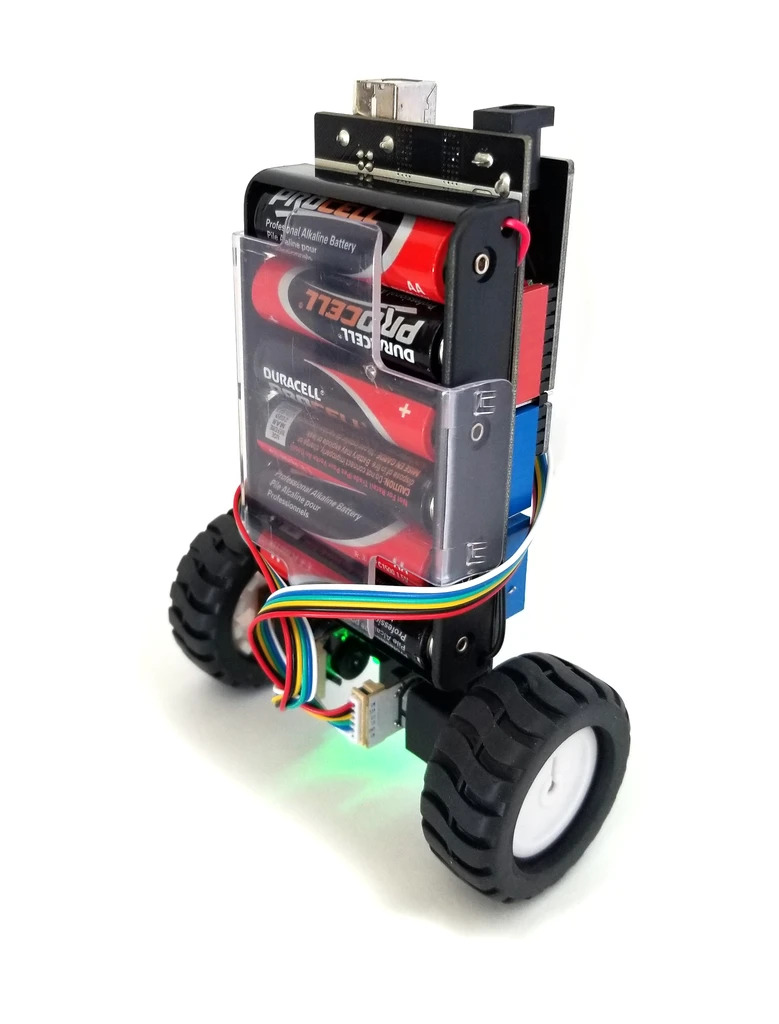
\includegraphics[height = 5.5cm]{minseg-M2V5}
	\end{center}
	\note<1-1>{\begin{itemize}
		\item 
	\end{itemize}}
\end{frame}


\begin{frame}{Table of contents}
	\tableofcontents
\end{frame}


% ~~~~~~~~~~~~~~~~~~~~~~~~~~~~~~~~~~~~~~~~~~~~~~~~~~~~~~~~~~~~~~~~~ %
\section{Installing the software}


\begin{frame}[t]{Instructions for installing the software: Arduino IDE}
	If you have not done so yet, download and install the latest Arduino IDE from \url{https://www.arduino.cc/en/Main/Software}, \\ it should look like this:
	\begin{center}
		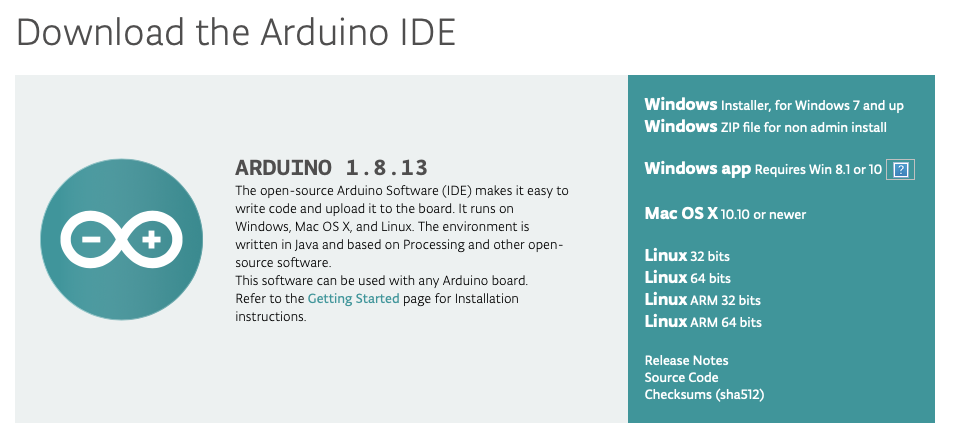
\includegraphics[width = 0.6\textwidth]{Screenshot_arduino_IDE}
	\end{center}
	Note that you might get a ``Windows Security'' message asking whether you would like to install the ``Adafruit Industries LLC Ports'' and ``Arduino USB Driver'' software too. In this case, install that as well.
\end{frame}


\begin{frame}[t]{Instructions for installing the software: Balancing Robot Project Software}
	Go to \url{https://github.com/justinlsquire/BalancingRobotsProject}, \\ it should look like this:
	\begin{center}
		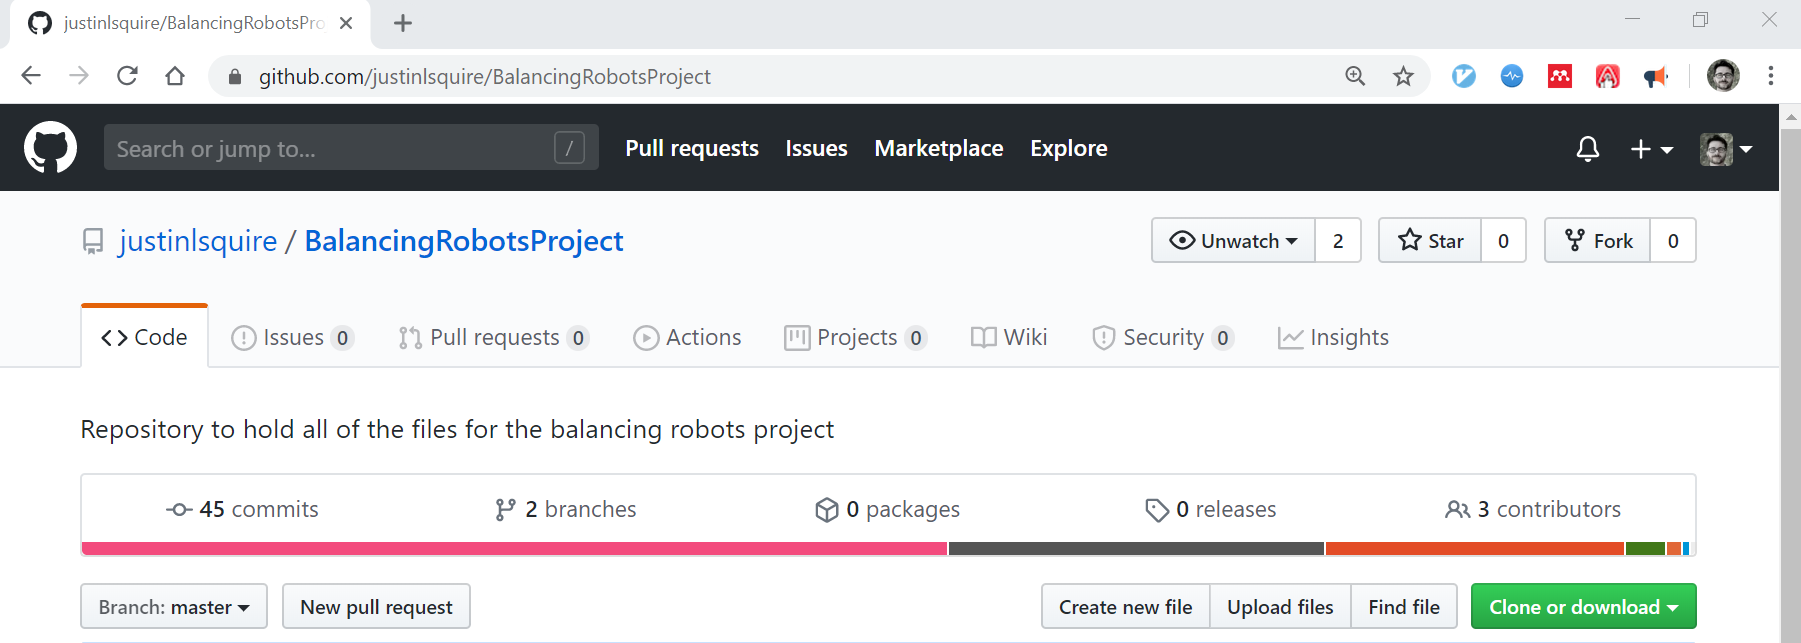
\includegraphics[width = 0.9\textwidth]{screenshot-github}
	\end{center}
\end{frame}


\begin{frame}[t]{Instructions for installing the software: Balancing Robot Project Software}
	Download the software by clicking the ``clone or download'' button:
	\begin{center}
		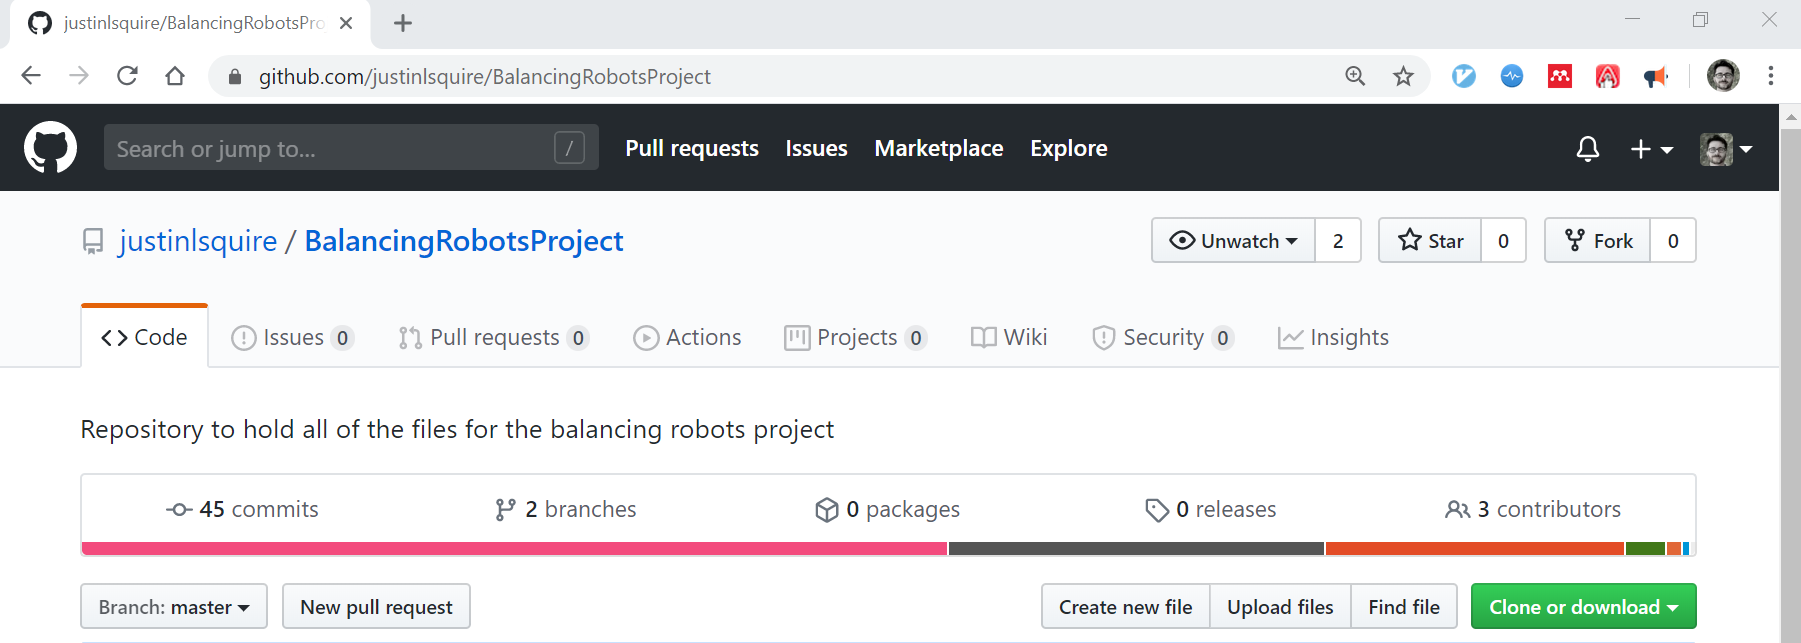
\includegraphics[width = 0.9\textwidth]{screenshot-github}
	\end{center}
	in any folder you prefer. Then unzip the downloaded file.
\end{frame}


\begin{frame}{Instructions for installing the software: Balancing Robot Project Software}
	Open the unzipped file (sometimes called also ``repository'') in your file explorer:
	\begin{center}
		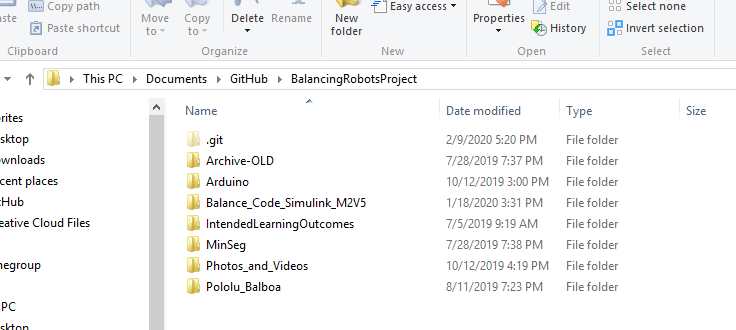
\includegraphics[width = 0.9\textwidth]{github-repository-explorer}
	\end{center}
\end{frame}


\begin{frame}{Instructions for installing the software: Balancing Robot Project Libraries}
	Go to the ``Arduino'' folder inside this just downloaded repository, then the ``libraries'' folder, then highlight and \BoldItPrimary{copy} the two folders called ``MINSEG\_V2'' and ``SEG\_CONTROL'':
	\begin{center}
		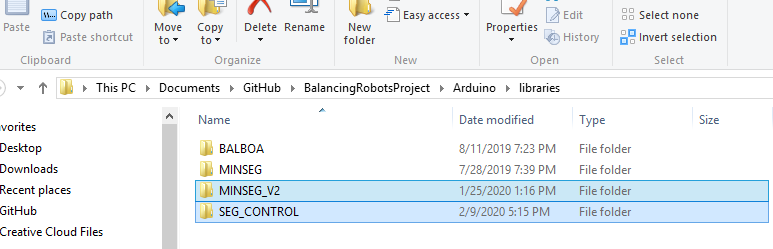
\includegraphics[width = 0.9\textwidth]{github-repository-explorer-2}
	\end{center}
\end{frame}


\begin{frame}{Instructions for installing the software: Balancing Robot Project Libraries}
Go to your Arduino Libraries folder (note that the default location for Windows is \texttt{Documents $\mapsto$ Arduino $\mapsto$ Libraries}. Sometimes is also \texttt{C:\textbackslash Program Files (x86) \textbackslash Arduino \textbackslash libraries}) and paste the two folders there:
	\begin{center}
		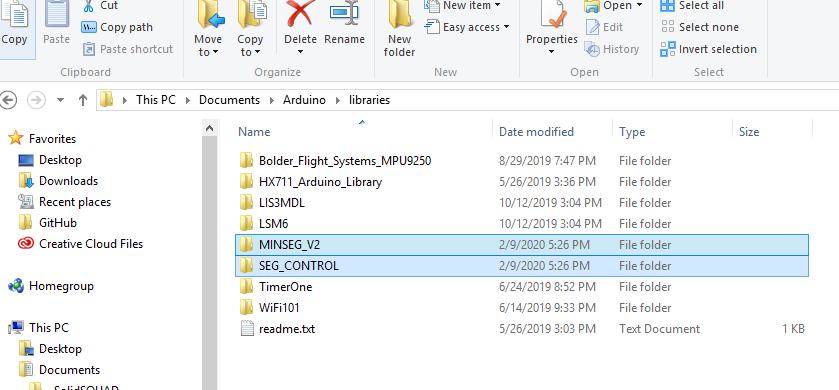
\includegraphics[width = 0.9\textwidth]{github-repository-explorer-3}
	\end{center}
\end{frame}

% ~~~~~~~~~~~~~~~~~~~~~~~~~~~~~~~~~~~~~~~~~~~~~~~~~~~~~~~~~~~~~~~~~ %
\begin{frame}{Table of contents}
	\tableofcontents
\end{frame}

% ~~~~~~~~~~~~~~~~~~~~~~~~~~~~~~~~~~~~~~~~~~~~~~~~~~~~~~~~~~~~~~~~~ %
\section{Connecting the robot}
\begin{frame}{Connecting the robot: Connect the hardware}
	\begin{itemize}
		\item Add six AA batteries to the back of the robot.
		\item Use the usb cable to connect the robot to your computer. 
		\item Switch the ``Driver Enable'' switch in the top left corner of the robot to ``off''.
		\end{itemize}
\end{frame}

\begin{frame}{Connecting the robot: Open the file}
	Go back to the GitHub repository folder \texttt{BalancingRobotsProject $\mapsto$ Arduino $\mapsto$ Minseg\_test\_M2V5}, and then open the ``Minseg\_test\_M2V5.ino'' file in Arduino (it should be fine to just double click on it, since the extension ``.ino'' should now be associated to the Arduino IDE program)
	\begin{center}
		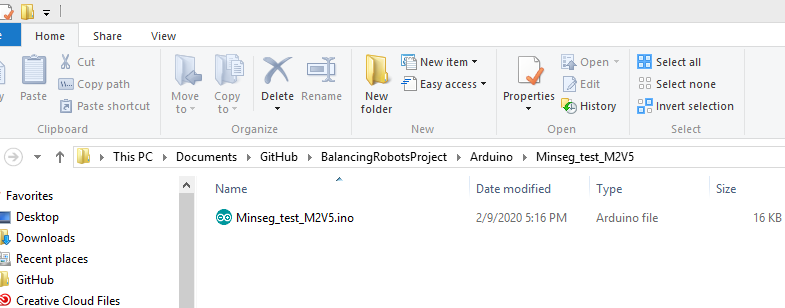
\includegraphics[width = 0.8\textwidth]{github-repository-explorer-minseg-test}
	\end{center}
	If it is the first time that you open this type of file you may get some firewall alerts about javaw.exe. Allow access
\end{frame}


\begin{frame}{Connecting the robot: Select the board}
	Go to \texttt{Tools $\mapsto$ Board} and select ``Arduino/Genuino Mega or Mega 2560'' (sometimes one may have only ``Arduino Mega or Mega 2560''; that is ok too!)
	\begin{center}
		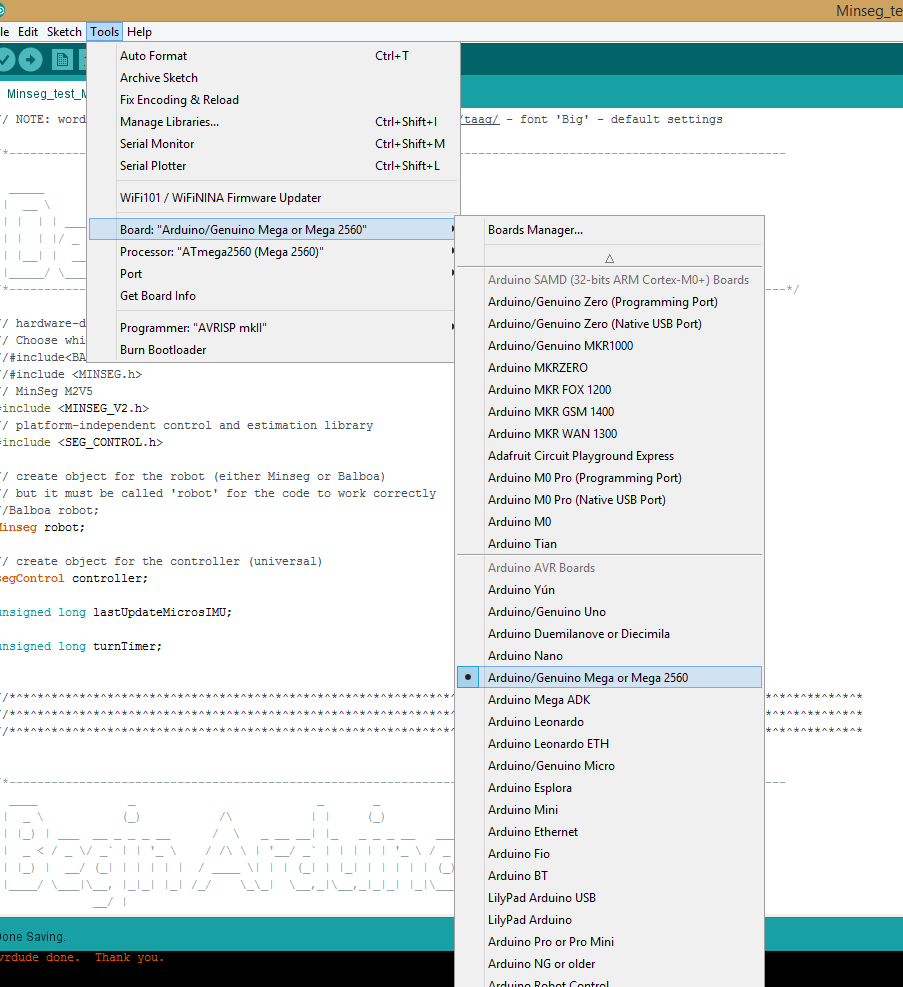
\includegraphics[width = 0.5\textwidth]{arduino-board-manager}
	\end{center}
\end{frame}


\begin{frame}{Connecting the robot: Select the port}
	Go to \texttt{Tools $\mapsto$ Port} and select the COM port associated with the MinSeg you plugged in via the USB port. (If you unplug the MinSeg and check this Port field again, you should see one missing\ldots This is the port that you should select when you plug back in the MinSeg.)
	\begin{center}
		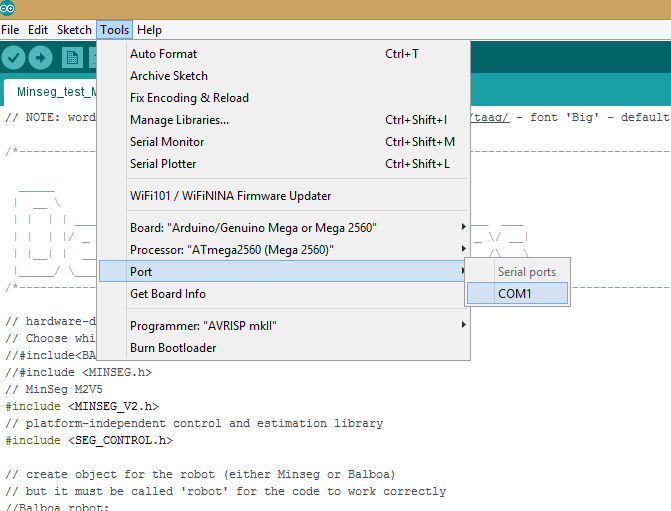
\includegraphics[width = 0.5\textwidth]{arduino-board-tool}
	\end{center}
\end{frame}

% ~~~~~~~~~~~~~~~~~~~~~~~~~~~~~~~~~~~~~~~~~~~~~~~~~~~~~~~~~~~~~~~~~ %
\begin{frame}{Table of contents}
	\tableofcontents
\end{frame}

% ~~~~~~~~~~~~~~~~~~~~~~~~~~~~~~~~~~~~~~~~~~~~~~~~~~~~~~~~~~~~~~~~~ %
\section{Calibrating the sensors}

\begin{frame}{Calibrating the sensors: Open the code}
	Find the right part of code for the calibration of the robot entitled
	\texttt{Sensor calibration steps}
	\begin{center}
		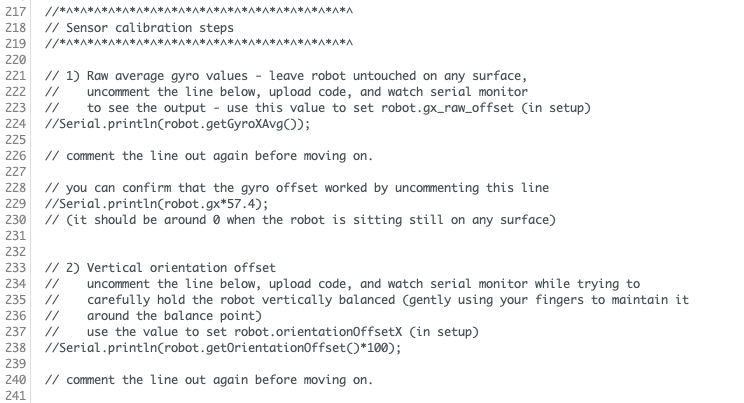
\includegraphics[width = 0.5\textwidth]{Screenshot_calibration_section}
	\end{center}
	The calibration routine is written out / explained in the code as well. So, we are basically going to follow these instructions step by step.
\end{frame}



\begin{frame}{Calibrating the sensors: First step: raw offset}
	Uncomment line 224 (or search for the line in case it has moved) so that it reads \texttt{Serial.println(robot.getGyroXAvg());} (without // !!)
	\begin{center}
		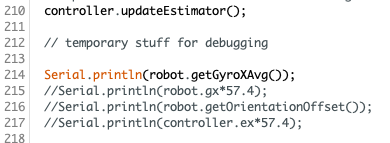
\includegraphics[width = 0.7\textwidth]{Screenshot_rawdataplot}
	\end{center}
	This will ensure that the raw data of the gyroscope can be read.
\end{frame}

%- save
%- upload the code as said in the next session
%- open the plotter and select the baud rate, use 115200 (in the bottom left of the window)
%
%
%140
%
%
%-1.68
%
%if you do not see well the balancing number then do 
%  Serial.println(100 * robot.getOrientationOffset());


\begin{frame}{Calibrating the sensors: Put the Minseg down}
	Put the Minseg onto a flat surface and let it lay absolutely still.
\end{frame}

\begin{frame}{Calibrating the sensors: Upload the code}
	Click the ``Upload'' button to load the code to the MinSeg
	\begin{center}
		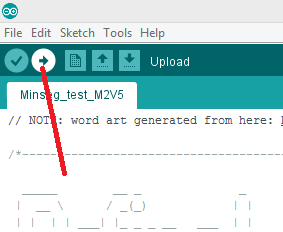
\includegraphics[width = 0.5\textwidth]{arduino-board-manager-upload}
	\end{center}
\end{frame}

\begin{frame}{Calibrating the sensors: Open the Serial plotter}
	Open the serial plotter by selecting the appropriate item in Tools.
	\begin{center}
		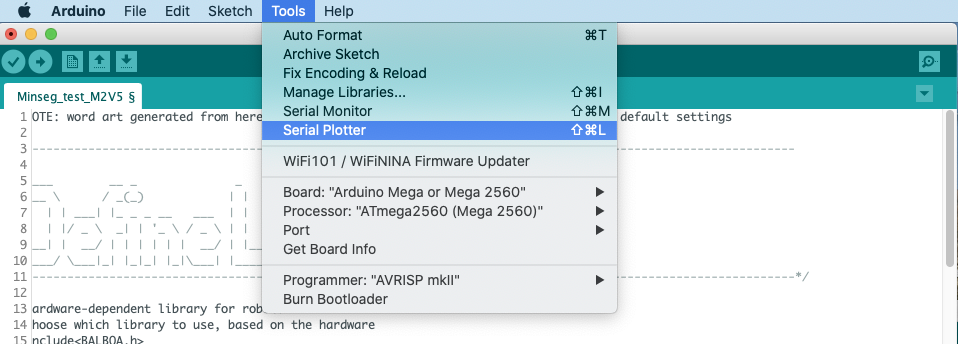
\includegraphics[width = 0.9\textwidth]{Screenshot_open_plotter}
	\end{center}
\end{frame}

\begin{frame}{Calibrating the sensors: Observe the raw measurement}
	Observe the values / the curve and note down the average value. (Here: roughly 372)
	\begin{center}
		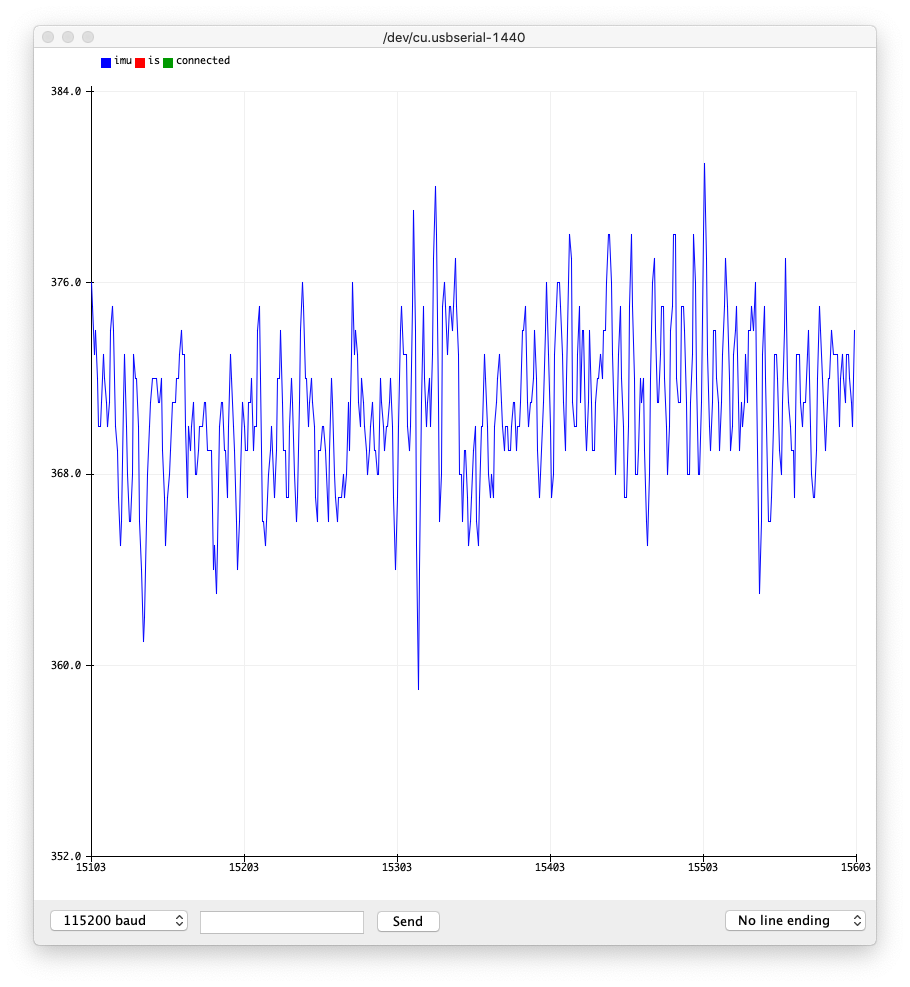
\includegraphics[width = 0.4\textwidth]{Screenshot_view_rawoffset}
	\end{center}
	Make sure to select ``115200 baud'' in the box at the bottom left of the plot window!
\end{frame}

\begin{frame}{Calibrating the sensors: Set the raw offset}
	Comment line 224 again so that it reads \texttt{//Serial.println(robot.getGyroXAvg());}.\\
	Find the line of code setting the gyro offset, which reads\\
	\texttt{robot.gx\_raw\_offset = 373; // gyro offset in raw units}\\
	and replace the offset value with the average that you observed above.
	\begin{center}
		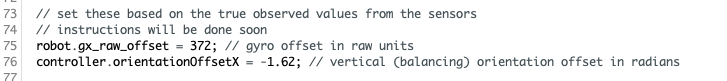
\includegraphics[width = 0.9\textwidth]{Screenshot_set_raw_offset}
	\end{center}
\end{frame}

\begin{frame}{Calibrating the sensors: Test the raw offset}
	Test whether the setting of the raw offset is correct by uncommenting line 229 so that it reads
	\texttt{Serial.println(robot.gx*57.4);}
	\begin{center}
		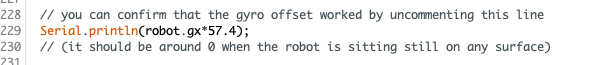
\includegraphics[width = 0.9\textwidth]{Screenshot_rawoffset_test}
	\end{center}
	upload the code to the Minseg, place it still on a flat surface and observe the values in the serial plotter.\\
	If the calibration was successful, the plotted values should be around 0. Comment line 229 afterwards again.
\end{frame}

\begin{frame}{Calibrating the sensors: Second step: orientation offset}
	Uncomment line 238 (or search for the line in case it has moved) so that it reads \texttt{Serial.println(robot.getOrientationOffset()*100);} (without // !!)
	\begin{center}
		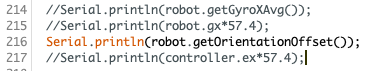
\includegraphics[width = 0.9\textwidth]{Screenshot_oreintation_offset}
	\end{center}
	NOTE: This plots the value times a factor of 100 (!!) to allow to see the usually small value in more detail / higher resolution.
\end{frame}

\begin{frame}{Calibrating the sensors: Observe the orientation offset}
	Similar to observing the raw offset,
	\begin{itemize}
		\item save the code (ctrl-S)
		\item Upload the code to the Minseg.
		\item Open the serial plotter.
		\item Hold the Minseg carefully between your finger tips so that it balances!!
		\item Observe the value when the robot is still and balances and note the average value.
		\item In line 76, set \texttt{controller.orientationOffsetX} to the value you observed divided by 100 (!!) .
		\item Comment line 238 again.
		\item Save the code again (ctrl-S)
		\end{itemize}
\end{frame}

\begin{frame}{Calibrating the sensors: Test the orientation offset}
	Test whether the setting of the orientation offset is correct by uncommenting line 243 so that it reads
	\texttt{Serial.println(controller.ex*57.4);}
	\begin{center}
		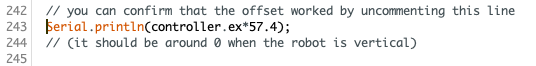
\includegraphics[width = 0.9\textwidth]{Screenshot_orientationoffset_test}
	\end{center}
	upload the code to the Minseg, hold it carefully so that it balances and observe the values in the serial plotter.\\
	If the calibration was successful, the plotted values should be around 0. Comment line 243 afterwards again and save the code.
\end{frame}


% ~~~~~~~~~~~~~~~~~~~~~~~~~~~~~~~~~~~~~~~~~~~~~~~~~~~~~~~~~~~~~~~~~ %
\begin{frame}{Table of contents}
	\tableofcontents
\end{frame}

% ~~~~~~~~~~~~~~~~~~~~~~~~~~~~~~~~~~~~~~~~~~~~~~~~~~~~~~~~~~~~~~~~~ %
\section{Running the software}

\begin{frame}{Running the software: Upload the code including your calibrated values}
	Click the ``Upload'' button to load the code to the MinSeg
	\begin{center}
		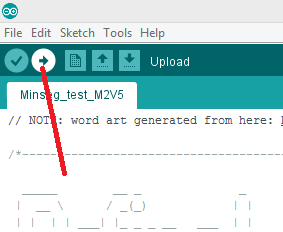
\includegraphics[width = 0.5\textwidth]{arduino-board-manager-upload}
	\end{center}
\end{frame}





\begin{frame}{Running the software: See the robot balance!}

	%explain that now you first upload, then remove the cable, then move the switches, explain what each switch does so that people will understand

	Hold the robot upright and make sure the switches are set to ``ON'', ``BATT'', and ``ON'' from the top down - the robot should start balancing if everything went well!
\end{frame}


%explain that if one wants to re-upload the code from Arduino IDE there is the need to re-put the switch ``driver voltage'' back



% ~~~~~~~~~~~~~~~~~~~~~~~~~~~~~~~~~~~~~~~~~~~~~~~~~~~~~~~~~~~~~~~~~ %
\end{document}														%
% ~~~~~~~~~~~~~~~~~~~~~~~~~~~~~~~~~~~~~~~~~~~~~~~~~~~~~~~~~~~~~~~~~ %
% ./FramesTemplates/template__citation.tex
% ./FramesTemplates/template__empty_frame.tex
% ./FramesTemplates/template__frame_with_blocks.tex
% ./FramesTemplates/template__frame_with_colored_background.tex
% ./FramesTemplates/template__frame_with_itemized_list.tex
% ./FramesTemplates/template__frame_with_overlayed_figures.tex
% ./FramesTemplates/template__frame_with_two_columns.tex
% ./FramesTemplates/template__frame_with_two_columns_and_overlayed_figures.tex


\begin{frame}{}{}
	
	\note<1-1>{\begin{itemize}
		\item 
	\end{itemize}}
\end{frame}




